\documentclass[aspectratio=169]{beamer}
\usepackage{graphicx}
\usepackage{hyperref}
\usepackage[utf8]{inputenc}
\usepackage[T1]{fontenc}
\usepackage{tikz}
\usepackage{listings}
\usepackage{xcolor}
\usepackage{amsmath}
\usepackage{amssymb}

% Theme setup
\usetheme{Madrid}
\usecolortheme{seahorse}

% Title information
\title{Sample Beamer Presentation}
\subtitle{A Comprehensive Demo of LaTeX Beamer Features}
\author{Dr. Jane Smith}
\institute{University of Technology}
\date{\today}

\begin{document}

% Title slide
\begin{frame}
\titlepage
\end{frame}

% Table of contents
\begin{frame}{Outline}
\tableofcontents
\end{frame}

% Section 1: Introduction
\section{Introduction}

\begin{frame}{What is Beamer?}
\begin{itemize}
    \item A LaTeX document class for creating presentations
    \item Supports overlays, animations, and transitions
    \item Perfect for academic and technical presentations
    \item Produces high-quality PDF output
\end{itemize}

\begin{block}{Key Features}
Beamer provides professional themes, automatic numbering, and seamless integration with LaTeX's mathematical typesetting.
\end{block}
\end{frame}

\begin{frame}{Why Use LaTeX for Presentations?}
\begin{columns}
\column{0.5\textwidth}
\textbf{Advantages:}
\begin{itemize}
    \item Consistent formatting
    \item Superior math support
    \item Version control friendly
    \item Cross-platform
\end{itemize}

\column{0.5\textwidth}
\textbf{Use Cases:}
\begin{itemize}
    \item Academic conferences
    \item Technical talks
    \item Research presentations
    \item Teaching materials
\end{itemize}
\end{columns}
\end{frame}

% Section 2: Text and Formatting
\section{Text and Formatting}

\begin{frame}{Text Formatting Options}
\begin{itemize}
    \item \textbf{Bold text} for emphasis
    \item \textit{Italic text} for definitions
    \item \underline{Underlined text} for highlighting
    \item \texttt{Monospace text} for code
    \item \textcolor{red}{Colored text} for visual appeal
\end{itemize}

\vspace{0.5cm}

\begin{alertblock}{Important Note}
Beamer supports all standard LaTeX formatting commands and provides additional presentation-specific features.
\end{alertblock}
\end{frame}

\begin{frame}{Lists and Enumerations}
\begin{columns}
\column{0.5\textwidth}
\textbf{Itemize Lists:}
\begin{itemize}
    \item First level
    \begin{itemize}
        \item Second level
        \begin{itemize}
            \item Third level
        \end{itemize}
    \end{itemize}
    \item Back to first level
\end{itemize}

\column{0.5\textwidth}
\textbf{Enumerate Lists:}
\begin{enumerate}
    \item First point
    \item Second point
    \begin{enumerate}
        \item Sub-point A
        \item Sub-point B
    \end{enumerate}
    \item Third point
\end{enumerate}
\end{columns}
\end{frame}

% Section 3: Mathematics
\section{Mathematical Content}

\begin{frame}{Mathematical Equations}
\begin{block}{Inline Mathematics}
The quadratic formula $x = \frac{-b \pm \sqrt{b^2 - 4ac}}{2a}$ is fundamental to algebra.
\end{block}

\begin{block}{Display Mathematics}
\begin{equation}
\int_{-\infty}^{\infty} e^{-x^2} dx = \sqrt{\pi}
\end{equation}
\end{block}

\begin{block}{Aligned Equations}
\begin{align}
f(x) &= x^2 + 2x + 1 \\
f'(x) &= 2x + 2 \\
f''(x) &= 2
\end{align}
\end{block}
\end{frame}

\begin{frame}{Mathematical Theorems}
\begin{theorem}[Pythagorean Theorem]
For a right triangle with legs $a$ and $b$ and hypotenuse $c$:
\[a^2 + b^2 = c^2\]
\end{theorem}

\begin{proof}
Consider a square with side length $(a+b)$ and rearrange the areas to demonstrate the relationship.
\end{proof}

\begin{corollary}
If $a = b = 1$, then $c = \sqrt{2}$.
\end{corollary}
\end{frame}

% Section 4: Images and Graphics
\section{Images and Graphics}

\begin{frame}{Including Images}
\begin{center}
\includegraphics[width=0.3\textwidth]{images/sample_chart.png}
\end{center}

\begin{itemize}
    \item Images can be resized using width and height parameters
    \item Supported formats: PDF, PNG, JPG, EPS
    \item Images can be centered, left-aligned, or right-aligned
\end{itemize}

\begin{exampleblock}{Example}
The chart above shows sample data visualization capabilities.
\end{exampleblock}
\end{frame}

\begin{frame}{Multiple Images}
\begin{columns}
\column{0.33\textwidth}
\begin{center}
\includegraphics[width=\textwidth]{images/diagram1.png}\\
\small{Figure 1: System Architecture}
\end{center}

\column{0.33\textwidth}
\begin{center}
\includegraphics[width=\textwidth]{images/diagram2.png}\\
\small{Figure 2: Data Flow}
\end{center}

\column{0.33\textwidth}
\begin{center}
\includegraphics[width=\textwidth]{images/diagram3.png}\\
\small{Figure 3: Results}
\end{center}
\end{columns}

\vspace{0.5cm}
\begin{center}
\textit{Three different visualization approaches for the same dataset.}
\end{center}
\end{frame}

% Section 5: Tables
\section{Tables and Data}

\begin{frame}{Data Tables}
\begin{table}
\centering
\begin{tabular}{|l|c|r|}
\hline
\textbf{Algorithm} & \textbf{Time Complexity} & \textbf{Space Complexity} \\
\hline
Bubble Sort & $O(n^2)$ & $O(1)$ \\
Quick Sort & $O(n \log n)$ & $O(\log n)$ \\
Merge Sort & $O(n \log n)$ & $O(n)$ \\
Heap Sort & $O(n \log n)$ & $O(1)$ \\
\hline
\end{tabular}
\caption{Comparison of Sorting Algorithms}
\end{table}

\begin{itemize}
    \item Tables can include mathematical expressions
    \item Column alignment can be specified
    \item Borders and rules can be customized
\end{itemize}
\end{frame}

% Section 6: Code Listings
\section{Code Examples}

\begin{frame}[fragile]{Code Listings}
\begin{block}{Python Example}
\begin{lstlisting}[language=Python]
def fibonacci(n):
    if n <= 1:
        return n
    return fibonacci(n-1) + fibonacci(n-2)

# Calculate first 10 Fibonacci numbers
for i in range(10):
    print(f"F({i}) = {fibonacci(i)}")
\end{lstlisting}
\end{block}

\begin{itemize}
    \item Syntax highlighting for multiple languages
    \item Line numbers can be added
    \item Code can be formatted within blocks
\end{itemize}
\end{frame}

% Section 7: TikZ Graphics
\section{TikZ Graphics}

\begin{frame}{TikZ Diagrams}
\begin{center}
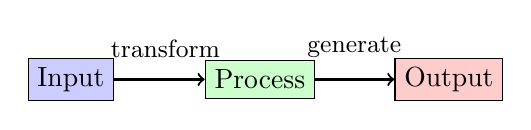
\begin{tikzpicture}[scale=0.8]
    % Nodes
    \node[draw, rectangle, fill=blue!20] (input) at (0,0) {Input};
    \node[draw, rectangle, fill=green!20] (process) at (3,0) {Process};
    \node[draw, rectangle, fill=red!20] (output) at (6,0) {Output};

    % Arrows
    \draw[->, thick] (input) -- (process);
    \draw[->, thick] (process) -- (output);

    % Labels
    \node[above] at (1.5, 0.2) {\small transform};
    \node[above] at (4.5, 0.2) {\small generate};
\end{tikzpicture}
\end{center}

\begin{itemize}
    \item TikZ allows creation of custom graphics directly in LaTeX
    \item Diagrams are vector-based and scale perfectly
    \item Integrates seamlessly with mathematical notation
\end{itemize}
\end{frame}

% Section 8: Overlays and Animations
\section{Advanced Features}

\begin{frame}{Overlays and Progressive Display}
\begin{itemize}
    \item<1-> This appears on all slides
    \item<2-> This appears starting from slide 2
    \item<3-> This appears starting from slide 3
    \item<4-> This appears starting from slide 4
\end{itemize}

\only<5>{
\begin{block}{Final Point}
Overlays allow you to control when content appears, creating a dynamic presentation effect.
\end{block}
}
\end{frame}

\begin{frame}{Column Layouts}
\begin{columns}[T]
\column{0.45\textwidth}
\begin{block}{Left Column}
\begin{itemize}
    \item Point A
    \item Point B
    \item Point C
\end{itemize}
\end{block}

\column{0.45\textwidth}
\begin{alertblock}{Right Column}
\begin{enumerate}
    \item First
    \item Second
    \item Third
\end{enumerate}
\end{alertblock}
\end{columns}

\vspace{0.5cm}
\begin{center}
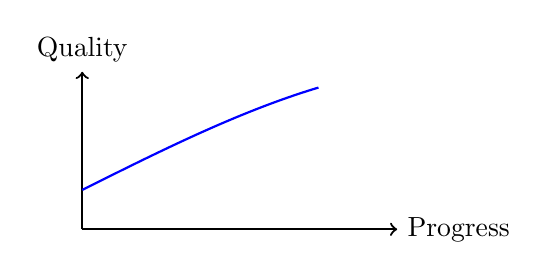
\begin{tikzpicture}
    \draw[thick, ->] (0,0) -- (4,0) node[right] {Progress};
    \draw[thick, ->] (0,0) -- (0,2) node[above] {Quality};
    \draw[blue, thick] (0,0.5) .. controls (1,1) and (2,1.5) .. (3,1.8);
\end{tikzpicture}
\end{center}
\end{frame}

% Section 9: Conclusion
\section{Conclusion}

\begin{frame}{Summary}
\begin{itemize}
    \item \textbf{Text Formatting}: Bold, italic, colors, and more
    \item \textbf{Mathematics}: Superior equation typesetting
    \item \textbf{Graphics}: Images, TikZ diagrams, and charts
    \item \textbf{Code}: Syntax-highlighted listings
    \item \textbf{Layouts}: Columns, blocks, and overlays
    \item \textbf{Themes}: Professional presentation styles
\end{itemize}

\vspace{0.5cm}

\begin{block}{Key Takeaway}
LaTeX Beamer provides everything needed for professional technical presentations with the power and consistency of the LaTeX typesetting system.
\end{block}
\end{frame}

\begin{frame}{Thank You!}
\begin{center}
\Large{Questions and Discussion}

\vspace{1cm}

\includegraphics[width=0.2\textwidth]{images/thank_you.png}

\vspace{1cm}

\normalsize
\texttt{jane.smith@university.edu}\\
\texttt{https://github.com/marvins/slide-forge}
\end{center}
\end{frame}

\end{document}
